% Spin-Wave Theory Overview
% Converted on 2026-10-08 from docs/lswt/00-foundations/lswt-overview.md (status: draft, source-section: "Introduction to Spin Wave Theory: model and workflow").
% Review status: draft; awaiting the user's physics and mathematics review.

\hypertarget{sec-lswt-lswt-overview}{%
\section{Spin-Wave Theory Overview}\label{sec-lswt-lswt-overview}}

Spin-wave theory (SWT) describes low-energy collective spin excitations and the associated quantum fluctuations about an ordered reference state. The nature of that reference state determines the appropriate formulation: local spin directions describe magnetically ordered or field-polarized states, whereas multipolar and bond-ordered phases require enlarged local or cluster reference states. Phases without a suitable semiclassical product reference require a different low-energy description.

For states described by local spin directions, SWT is most commonly formulated using SU(2) spin-coherent states and Holstein--Primakoff bosons. Linear spin-wave theory (LSWT) is the harmonic approximation obtained by retaining terms up to quadratic order in these bosons.

\begin{figure}
\centering
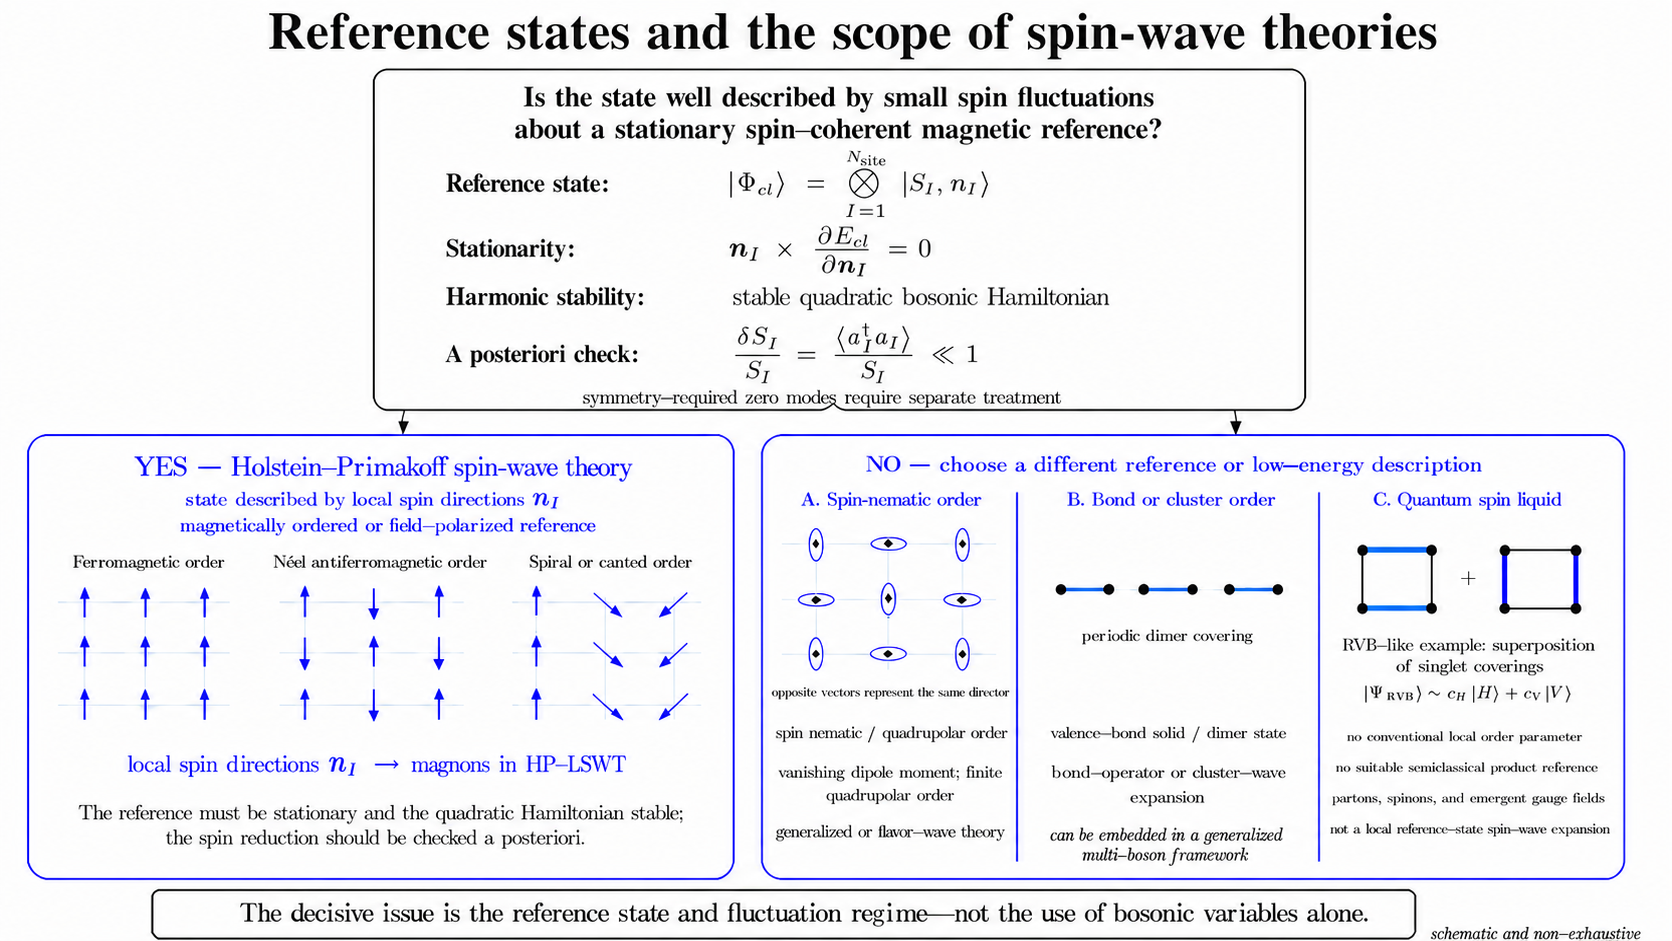
\includegraphics{figures/spin-wave-theory-classification.png}
\caption{Representative reference states and phases classified according to whether they admit a Holstein--Primakoff spin-coherent reference.}
\end{figure}

\emph{The classification is schematic and non-exhaustive. A compatible stationary reference and a stable quadratic Hamiltonian are prerequisites for Holstein--Primakoff LSWT, whereas a small spin reduction is an a posteriori check of the harmonic approximation.}

\subsection{Holstein--Primakoff Spin-Wave Theory}

For spin length \(S_I\) and a local unit vector \(\mathbf n_I\), the reference configuration is represented by the spin-coherent product state

\[
|\Phi_{\mathrm{cl}}[\{\mathbf n_I\}]\rangle
=
\bigotimes_I |S_I,\mathbf n_I\rangle,
\qquad
\langle\Phi_{\mathrm{cl}}|
\hat{\mathbf S}_I
|\Phi_{\mathrm{cl}}\rangle
=
S_I\mathbf n_I.
\]

The classical energy associated with this reference state is

\[
E_{\mathrm{cl}}[\{\mathbf n_I\}]
=
\langle\Phi_{\mathrm{cl}}[\{\mathbf n_I\}]|
\hat H
|\Phi_{\mathrm{cl}}[\{\mathbf n_I\}]\rangle.
\]

The product state is the semiclassical expansion point, not an assertion that the exact quantum state is unentangled or has an ordered moment of magnitude \(S_I\). The Holstein--Primakoff representation maps deviations from the local directions \(\mathbf n_I\) to bosons, and the quadratic Hamiltonian describes their collective normal modes as magnons. The local-frame construction and bosonic expansion are developed in Classical Order and Local Frame (Section~\ref{sec-lswt-classical-order-and-local-frame}) and \lswtnoteref{LSWT derivation}{Holstein–Primakoff Expansion}.

\subsection{Validity of Holstein--Primakoff LSWT}

The existence of a spin-coherent reference configuration permits a Holstein--Primakoff representation to be constructed, but it does not by itself establish that LSWT is an appropriate approximation. Its prerequisites and self-consistency check have different logical roles:

\begin{itemize}
\tightlist
\item
  \textbf{Reference compatibility:} the state of interest must admit a low-energy description in terms of fluctuations about a local spin-coherent configuration.
\item
  \textbf{Stationarity:} the reference configuration must satisfy \(\mathbf n_I\times\partial E_{\mathrm{cl}}/\partial\mathbf n_I=0\), so that no term linear in the fluctuation bosons remains.
\item
  \textbf{Harmonic stability:} the quadratic expansion must define a stable bosonic problem. The precise energetic and dynamical stability conditions, including the treatment of symmetry-required zero modes, belong to \lswtnoteref{LSWT derivation}{Paraunitary Diagonalization}.
\item
  \textbf{A posteriori self-consistency:} after diagonalization, the local spin reduction \(\delta S_I=\langle\hat a_I^\dagger\hat a_I\rangle\) should satisfy \(\delta S_I/S_I\ll1\) wherever the harmonic approximation is used.
\end{itemize}

Failure of a prerequisite invalidates Holstein--Primakoff LSWT about the selected reference, whereas a large spin reduction signals that neglected interaction terms may be important. Neither conclusion rules out every possible spin-wave description. The momentum-space derivation developed here also assumes a commensurate reference configuration with a finite magnetic unit cell; this is a restriction of that derivation rather than a general limitation of SWT.

In two dimensions, the finite-temperature interpretation requires an additional qualification. A short-range isotropic Heisenberg model cannot sustain spontaneous ferromagnetic or antiferromagnetic long-range order at nonzero temperature. Consequently, a thermodynamic ordered-state interpretation of finite-temperature LSWT requires a symmetry-breaking field, anisotropy that removes the relevant continuous spin-rotation symmetry, interlayer coupling, a finite-size or crossover scale, or another physical infrared cutoff.

\subsection{Reference States Beyond Local Magnetic Order}

States without a local magnetic direction require a different reference state. Spin-nematic states with quadrupolar order but no magnetic dipole moment provide a representative example. Flavor-wave theory enlarges the local state space and can describe quadrupolar or higher multipolar order. Bond-operator and cluster-wave theories instead expand about singlet dimers or larger local units. These approaches may retain a harmonic bosonic structure, but their fluctuation variables are not Holstein--Primakoff bosons about local spin directions. Multipolar moments can also coexist with magnetic dipole order, so the absence of a local spin direction is not a defining property of all multipolar phases.

A quantum spin liquid has no suitable semiclassical product reference for a local spin-wave expansion. Its low-energy description may instead involve fractionalized spinons and emergent gauge fields. The use of bosonic variables alone therefore does not determine whether a formulation is a spin-wave theory; the reference state and fluctuation expansion must also be specified.

\subsection{Bilinear Spin Hamiltonians}

The Hamiltonian considered in the subsequent derivation is at most bilinear in the spin operators and can be written as

\[
\hat H
=
\sum_{\ell=(I,J)\in\mathcal L}
\hat{\mathbf S}_I
\mathbin{\cdot}
\mathsf J_\ell
\mathbin{\cdot}
\hat{\mathbf S}_J
+
\sum_I
\hat{\mathbf S}_I
\mathbin{\cdot}
\mathsf D_I
\mathbin{\cdot}
\hat{\mathbf S}_I
-
\sum_I
\mathbf h_I
\mathbin{\cdot}
\hat{\mathbf S}_I.
\]

The inter-site matrix \(\mathsf J_\ell\) includes isotropic Heisenberg exchange, antisymmetric Dzyaloshinskii--Moriya interaction, and symmetric anisotropic exchange, including bond-dependent Kitaev-type couplings. The on-site matrix \(\mathsf D_I\) represents single-ion anisotropy, and \(\mathbf h_I\) is the Zeeman-energy coefficient determined by the applied field and the material-dependent \(g\)-tensor. Link orientation, counting conventions, and the relation between \(\mathbf h_I\), the applied field, and the \(g\)-tensor are defined in Bilinear Spin Hamiltonian (Section~\ref{sec-lswt-bilinear-spin-hamiltonian}).

Genuine higher-order interactions, such as inter-site biquadratic coupling and four-spin ring exchange, lie outside this bilinear Hamiltonian class. Spin-wave expansions can be constructed for such models, but the resulting harmonic coefficients must be derived from those interactions rather than inferred from the bilinear formulas above.

\subsection{References}

\subsubsection{Internal Documents}

\begin{itemize}
\tightlist
\item
  Notation and Conventions (Section~\ref{sec-lswt-notation-and-conventions}): defines the symbols, indices, geometry, and matrix typography used here.
\item
  Bilinear Spin Hamiltonian (Section~\ref{sec-lswt-bilinear-spin-hamiltonian}): defines the Hamiltonian support and link-counting convention.
\item
  Classical Order and Local Frame (Section~\ref{sec-lswt-classical-order-and-local-frame}): defines the reference configuration and local-frame convention.
\item
  \lswtnoteref{LSWT derivation}{Holstein–Primakoff Expansion}: defines the bosonic representation and harmonic truncation.
\item
  \lswtnoteref{LSWT derivation}{Real-Space Boson Hamiltonian}: derives the quadratic Hamiltonian in real space.
\item
  \lswtnoteref{LSWT derivation}{Momentum-Space BdG Hamiltonian}: defines the Fourier and Nambu conventions.
\item
  \lswtnoteref{LSWT derivation}{Paraunitary Diagonalization}: states the stability conditions and obtains the magnon modes.
\end{itemize}

\subsubsection{External Sources}

\begin{itemize}
\tightlist
\item
  T. Holstein and H. Primakoff, \href{https://doi.org/10.1103/PhysRev.58.1098}{\emph{Field Dependence of the Intrinsic Domain Magnetization of a Ferromagnet}}, \emph{Physical Review} \textbf{58}, 1098--1113 (1940), DOI: \texttt{10.1103/PhysRev.58.1098}: introduces the Holstein--Primakoff boson representation.
\item
  S. Toth and B. Lake, \href{https://doi.org/10.1088/0953-8984/27/16/166002}{\emph{Linear spin wave theory for single-\(Q\) incommensurate magnetic structures}}, \emph{Journal of Physics: Condensed Matter} \textbf{27}, 166002 (2015), DOI: \texttt{10.1088/0953-8984/27/16/166002}: formulates LSWT using local spin frames and discusses its small-fluctuation regime.
\item
  R. A. Muniz, Y. Kato, and C. D. Batista, \href{https://doi.org/10.1093/ptep/ptu109}{\emph{Generalized spin-wave theory: application to the bilinear-biquadratic model}}, \emph{Progress of Theoretical and Experimental Physics} \textbf{2014}, 083I01 (2014), DOI: \texttt{10.1093/ptep/ptu109}: distinguishes the SU(2) spin-coherent formulation from generalized spin-wave theories for multipolar states.
\item
  L. Balents, \href{https://doi.org/10.1038/nature08917}{\emph{Spin liquids in frustrated magnets}}, \emph{Nature} \textbf{464}, 199--208 (2010), DOI: \texttt{10.1038/nature08917}: reviews quantum spin liquids, fractionalized excitations, and emergent gauge fields.
\item
  S. Sachdev and R. N. Bhatt, \href{https://doi.org/10.1103/PhysRevB.41.9323}{\emph{Bond-operator representation of quantum spins: Mean-field theory of frustrated quantum Heisenberg antiferromagnets}}, \emph{Physical Review B} \textbf{41}, 9323--9329 (1990), DOI: \texttt{10.1103/PhysRevB.41.9323}: introduces the singlet--triplet bond-operator expansion used for dimerized quantum magnets.
\item
  K. Majumdar, D. Furton, and G. S. Uhrig, \href{https://doi.org/10.1103/PhysRevB.85.144420}{\emph{Effects of ring exchange interaction on the Néel phase of two-dimensional, spatially anisotropic, frustrated Heisenberg quantum antiferromagnet}}, \emph{Physical Review B} \textbf{85}, 144420 (2012), DOI: \texttt{10.1103/PhysRevB.85.144420}: provides a spin-wave treatment of a Hamiltonian containing four-spin ring exchange.
\item
  N. D. Mermin and H. Wagner, \href{https://doi.org/10.1103/PhysRevLett.17.1133}{\emph{Absence of Ferromagnetism or Antiferromagnetism in One- or Two-Dimensional Isotropic Heisenberg Models}}, \emph{Physical Review Letters} \textbf{17}, 1133--1136 (1966), DOI: \texttt{10.1103/PhysRevLett.17.1133}: establishes the absence of spontaneous ferro- or antiferromagnetic long-range order at nonzero temperature in the short-range isotropic one- and two-dimensional Heisenberg model.
\end{itemize}
